
{\actuality} 
The Fourth Industrial Revolution (Industry 4.0) is characterized by the integration of digital technologies into manufacturing and production systems, significantly transforming energy management and consumption. This transition, shown in figure~\cref{fig:industry4}, is particularly evident in the increased reliance on electrical energy as a key production resource, impacting both industrial and household consumers who are increasingly sensitive to the quality and stability of electrical energy supply \autocite{He_2022}.

\begin{figure}[ht]
    \centerfloat{
        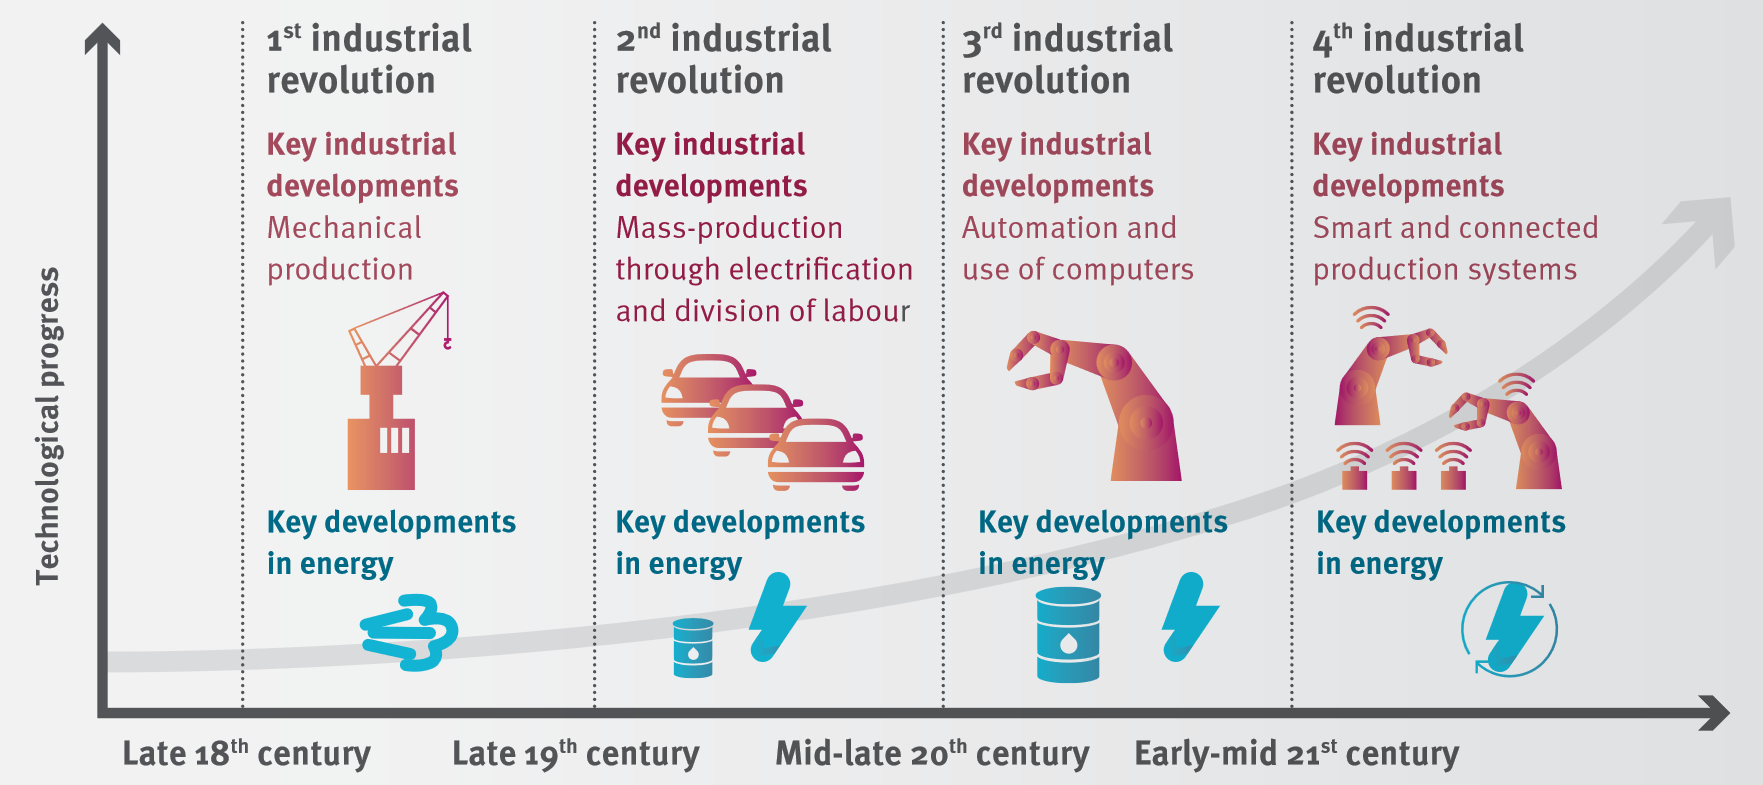
\includegraphics[scale=0.37]{industry4}
    }
    \caption{Industrial revolutions and key developments in energy change \cite{UNIDO2017}.}\label{fig:industry4}
\end{figure}

A new era of technological and social transformation is reshaping consumer expectations for energy systems, with the following required features \autocite{kholkin2025energy}:
\begin{itemize}
    \item  \textbf{Quality}: capability of power supply systems to meet the growing digital demand segment by delivering electricity with high reliability and performance standards, supported by energy storage systems (ESS), power electronics and digital control technologies.
    
    \item  \textbf{Autonomy}: energy resilience of settlements, individual consumers, mobile devices, and transport systems, enabled by local generation, storage, high-density energy conversion and smart grids, reducing reliance on centralized power and fuel supply.
    
    \item  \textbf{Intelligence}: digital modeling, scalable architectures, and digital markets enable dynamic energy exchange, automated control of complex infrastructure, and customized services to meet evolving demand.
\end{itemize}

\nomenclature{\(ESS\)}{Energy Storage Systems}


% \section{Challenges in microgrid operation and control}
\textbf{Challenges in microgrid operation and control.}
To satisfy consumer expectations, the global energy landscape is undergoing a significant transformation, driven by the increasing adoption of distributed energy systems that integrate various energy sources, including renewable generation (solar, wind), ESS, electric vehicles (EV) and controllable loads. Furthermore, the integration of renewable energy resources (RES) and distributed energy resources (DER) into the grid is typically achieved through inverter-based resources (IBR). The significant benefits of such systems in terms of energy security, sustainability, and economic efficiency, lead power grids to evolve into power electronics dominated grids (PEDG) \autocite{mag_ipakchi_2009}, as shown in figure~\cref{fig:bulk2pedg}. This transition results in an amplified complexity and significance for device and system-level control schemes to maintain resiliency, reliability and operational stability \autocite{mag_khan_2020}. 

\nomenclature{\(EV\)}{Electric Vehicles}
\nomenclature{\(PEDG\)}{Power Electronics Dominated Grid}
\nomenclature{\(DER\)}{Distributed Energy Resources}
\nomenclature{\(IBR\)}{Inverter-Based Resources}
\nomenclature{\(RES\)}{Renewable Energy Resources}

\begin{figure}[ht]
    \centerfloat{
        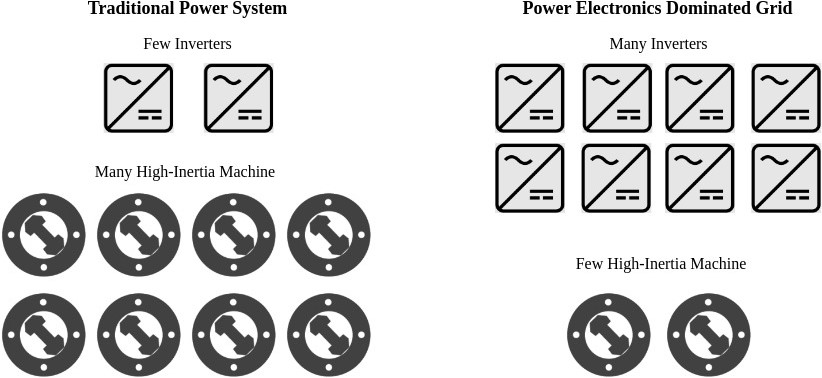
\includegraphics[scale=0.7]{bulk2pedg}
    }
    \caption{Transformation of energy paradigm.}\label{fig:bulk2pedg}
\end{figure}

As can be seen in figure~\cref{fig:pedg_time}, the characteristic time scale of power electronics devices ranges from microseconds to milliseconds, introducing rapid control loops for voltage, current and phase-locked loops (PLL) of the network inverters. In other words, PEDG has low mechanical inertia and rapid and multi-timescale dynamics \autocite{7182342}, while also considering the inherent stochastic nature of its energy resources.

\nomenclature{\(PLL\)}{Phase-Locked Loop}

The reduced presence of synchronous machines in PEDG compared to static power electronics-based generators has a substantial impact on system inertia. PEDG exhibit significantly lower inertia than bulk interconnected power systems. This low inertia, coupled with the low short-circuit capacity of the network, exacerbates the challenge of maintaining stability. Even minor deviations in PEDG architecture due to intentional load or generator disconnections can lead to drastic fluctuations in voltage and frequency. The mixture of synchronous machines and inverter-based generation units introduces a combination of large and small time constants in PEDG, potentially causing unintended shutdowns of inverter-based generation units during system perturbations.

\begin{figure}[ht]
    \centerfloat{
        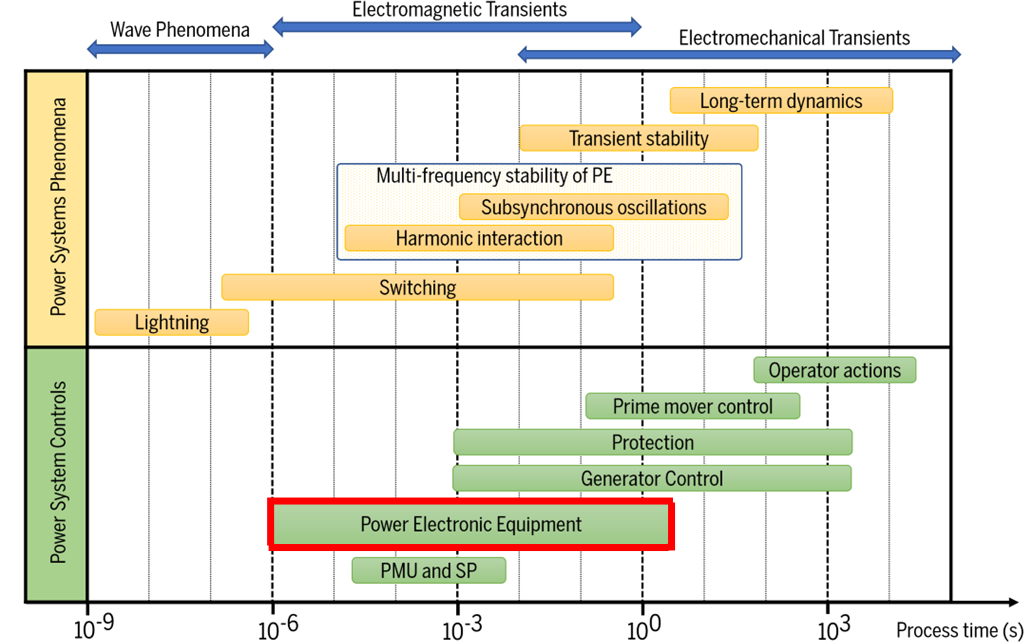
\includegraphics[scale=0.55]{pedg_time}
    }
    \caption{Characteristic operational time of PEDG \autocite{misc_karawita_2024}.}\label{fig:pedg_time}
\end{figure}

The intermittent nature of renewable energy sources in PEDG poses significant challenges for balancing demand and supply \autocite{7790991,7442160}. Moreover, the bidirectional power flow inherent in PEDG necessitates complex control and protection coordination among prosumers. It affects short-circuit current calculations and protection system design \autocite{4112346}, where engineers must consider the reserve for increased fault current magnitudes and the need to adjust protection settings to account for changed system characteristics. 

Furthermore, compared to the traditional bulk power system, PEDG exhibits unique characteristics due to the proximity of generation and load, resulting in shorter feeders and a lower inductance-resistance ratio (X/R) of grid impedance. In turn, it makes voltage control more challenging, requiring a careful management of reactive power \autocite{7749289}. 

Another key aspect, related with X/R ratio, is the equivalent impedance of the grid. The grid impedance plays a crucial role in determining the performance of IBRs. The performance of inverters is influenced not only by the inherent impedance of the power lines but also by the equivalent grid impedance at the Point of Common Coupling (PCC) as determined by the Thevenin equivalent circuit in figure~\cref{fig:thevenin}. This impedance can be altered by the connection of parallel-connected inverters, further impacting the operation of other grid-connected devices \autocite{Jayasinghe2021}.

\nomenclature{\(PCC\)}{Point of Common Coupling}

\begin{figure}[ht]
    \centerfloat{
        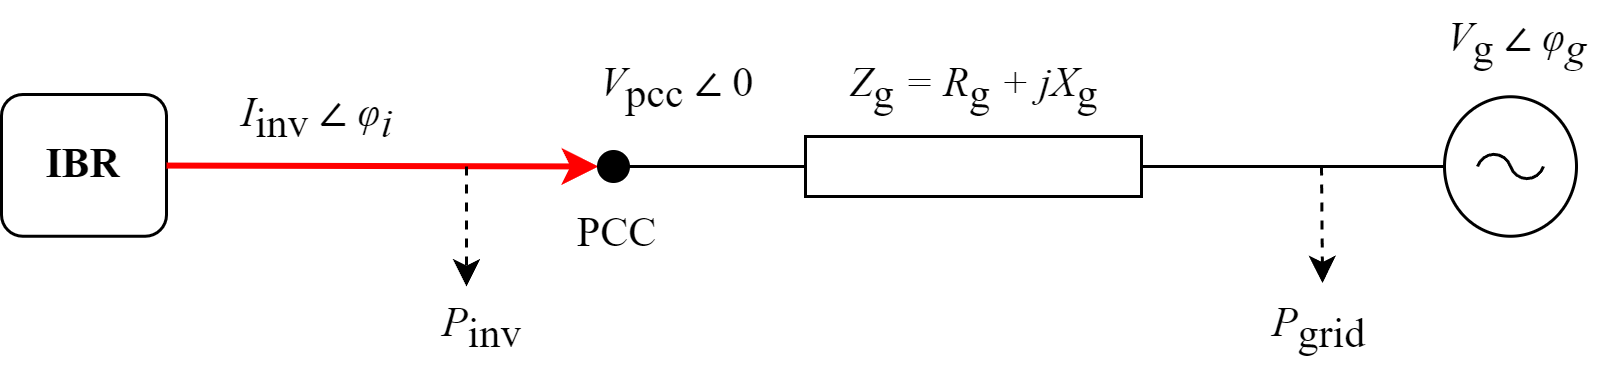
\includegraphics[scale=1.2]{thevenin}
    }
    \caption{Thevenin equivalent circuit of the grid-connected generation system.}\label{fig:thevenin}
\end{figure}

As the interconnection between multi-parallel inverters is established through the grid impedance, as shown in figure~\cref{fig:multi_parallel}, the connection or disconnection of an inverter induces changes in the impedance seen by other inverters. This can threaten the ability of the power system to return to its normal conditions after disturbance, which is the stability of these inverters \autocite{10615092}, what is particularly relevant for low-voltage distribution systems with a lot of DERs. The fast dynamics of IBRs along with the inverter system moving to stable or unstable region can be resulted in current oscillations, as shown in figure~\cref{fig:stability_regions}.

\begin{figure}[ht]
    \centerfloat{
        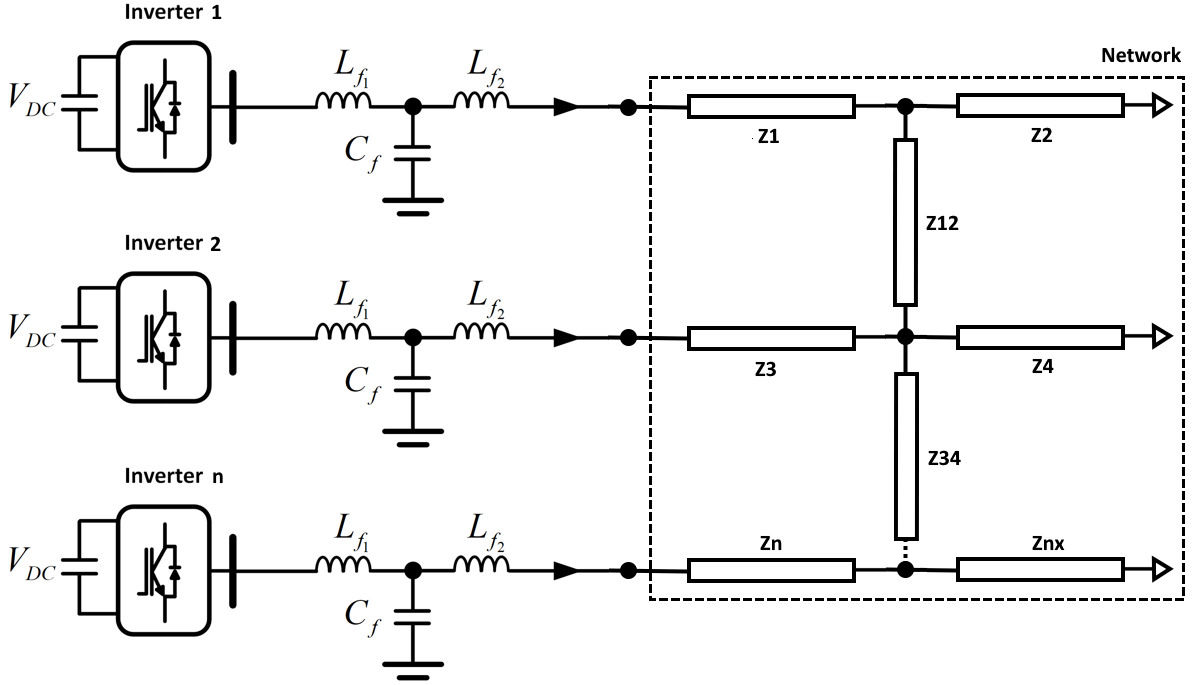
\includegraphics[scale=2]{multi_parallel}
    }
    \caption{Typical configuration of multiple paralleled inverters within a microgrid.}\label{fig:multi_parallel}
\end{figure}

\begin{figure}[ht]
    \centerfloat{
        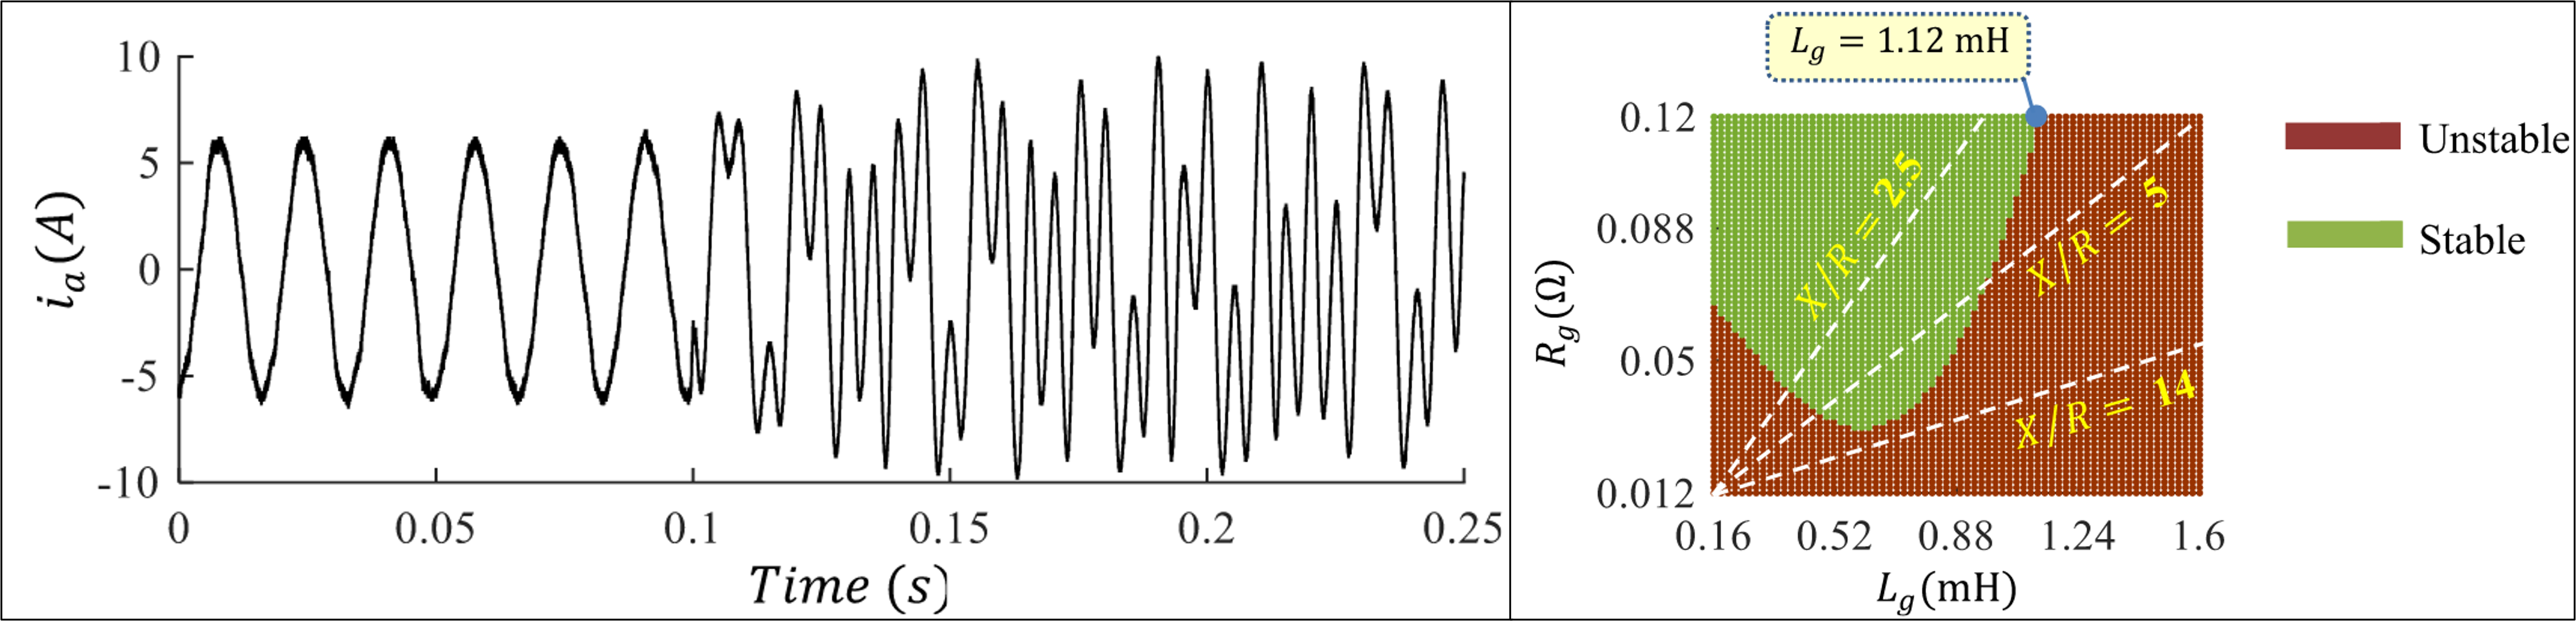
\includegraphics[scale=0.5]{stability_reg}
    }
    \caption{The stable and unstable regions with respect to X/R ratio \cite{8242351}.}\label{fig:stability_regions}
\end{figure}

The transition to PEDGs, driven by the integration of distributed generation, EVs and storage systems, introduces significant operational challenges evolving from low inertia, rapid dynamics, bidirectional power flow and stochastic behavior. The European project MIGRATE has outlined in \autocite{MIGRATE2016} the primary technical challenges associated with the extensive integration of IBRs into the grid. These challenges are summarized in Table \ref{tab:power_system_issues}, which was generalized for different level of systems and presented in figure~\cref{fig:general_issues}  in \autocite{8809097}.

\begin{table} [htbp]
    \centering
    \begin{threeparttable}% выравнивание подписи по границам таблицы
        \caption{Ranked Issues in Power Systems}\label{tab:power_system_issues}%
        \begin{tabular}{| c || p{13cm} |}
            \hline
            \hline
                \textbf{Rank} & \textbf{Issue} \\ \hline
                1 & Decrease of inertia \\ \hline
                2 & Resonances due to cables and IBR \\ \hline
                3 & Reduction of transient stability margins \\ \hline
                4 & Missing or wrong participation of IBR-connected generators and loads in frequency containment \\ \hline
                5 & IBR Controller interaction with each other and passive AC components \\ \hline
                6 & Loss of devices in the context of fault-ride-through capability \\ \hline
                7 & Lack of reactive power \\ \hline
                8 & Introduction of new power oscillations and/or reduced damping of existing power oscillations \\ \hline
                9 & Excess of reactive power \\ \hline
                10 & Voltage dip-induced frequency dip \\ \hline
                11 & Altered static and dynamic voltage dependence of loads \\ \hline
            \hline
        \end{tabular}
    \end{threeparttable}
\end{table}

\begin{figure}[ht]
    \centerfloat{
        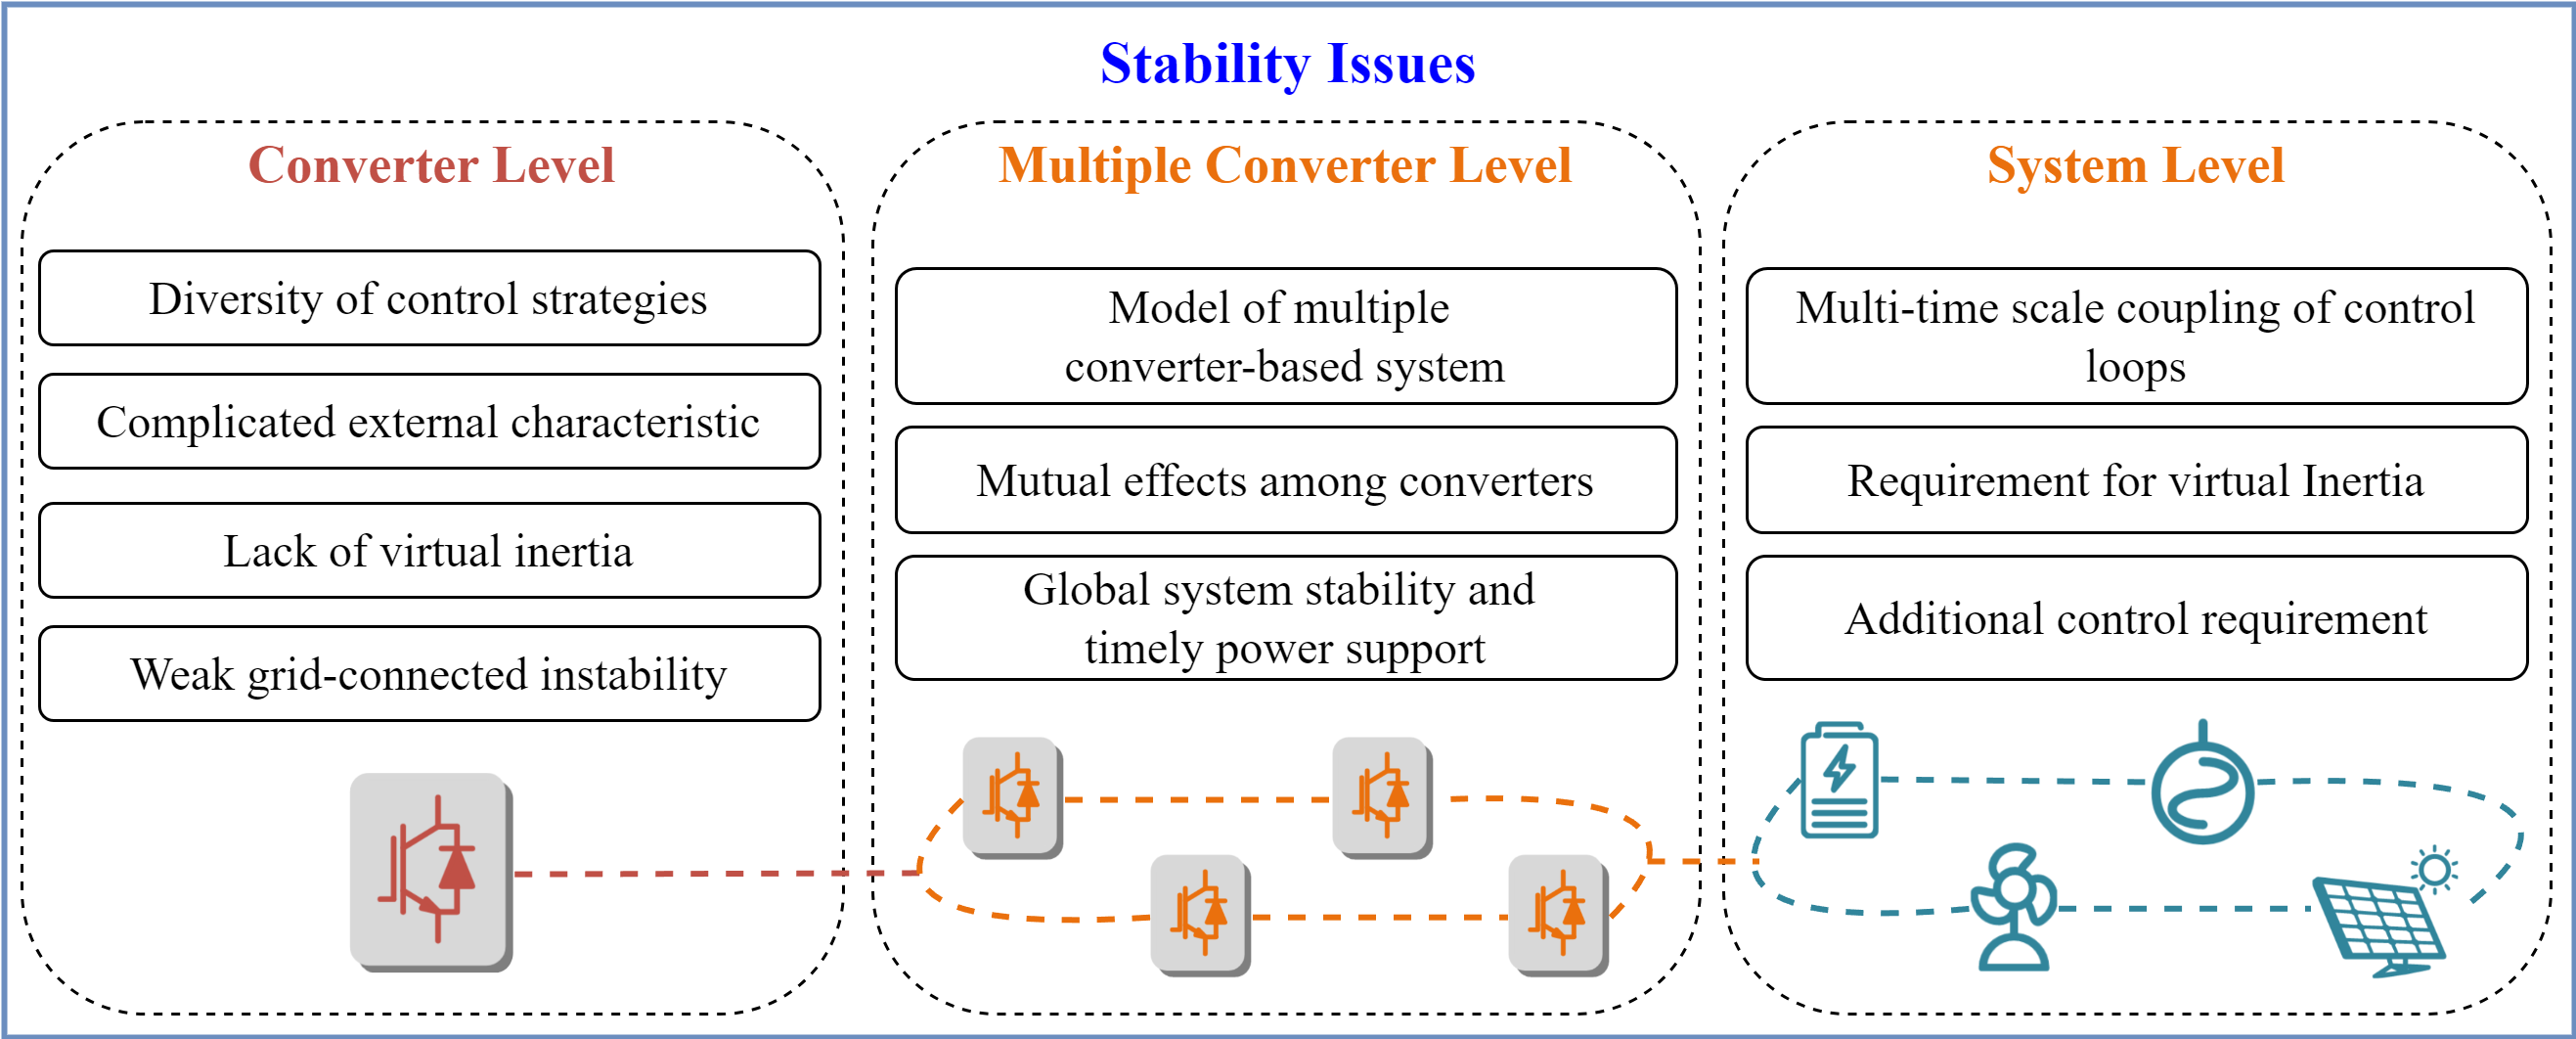
\includegraphics[scale=0.8]{general_issues}
    }
    \caption{General issues of PEDGs.}\label{fig:general_issues}
\end{figure}

Such characteristics require a paradigm shift in grid management, demanding real-time system awareness beyond the capabilities of traditional monitoring methods. The diverse timescales of PEDG dynamics, from microsecond-level converter control to minute-level demand-supply balancing, require fast and accurate dynamic state tracking to enable rapid instability detection, dynamic control and protection coordination, adaptive protection schemes, and optimized reactive power management. Maintaining secure operation of the system is one of the priority tasks, which critically depends on the system's overall observability.


\textbf{Need for Dynamic Mirroring.}
The electrical power system contains a transmission system, sub-transmission system, and distribution systems \cite{kundur1994power}. As can be seen from figure~\cref{fig:ps_illustration}, there is a comprehensive electrical interconnection among all components of the power system, whereas different voltage levels are interfaced by transformers. The fundamental role of a power system is to deliver electrical energy that meets predefined standards of quality, adequacy, reliability, and economic efficiency. 

\begin{figure}[ht]
    \centerfloat{
        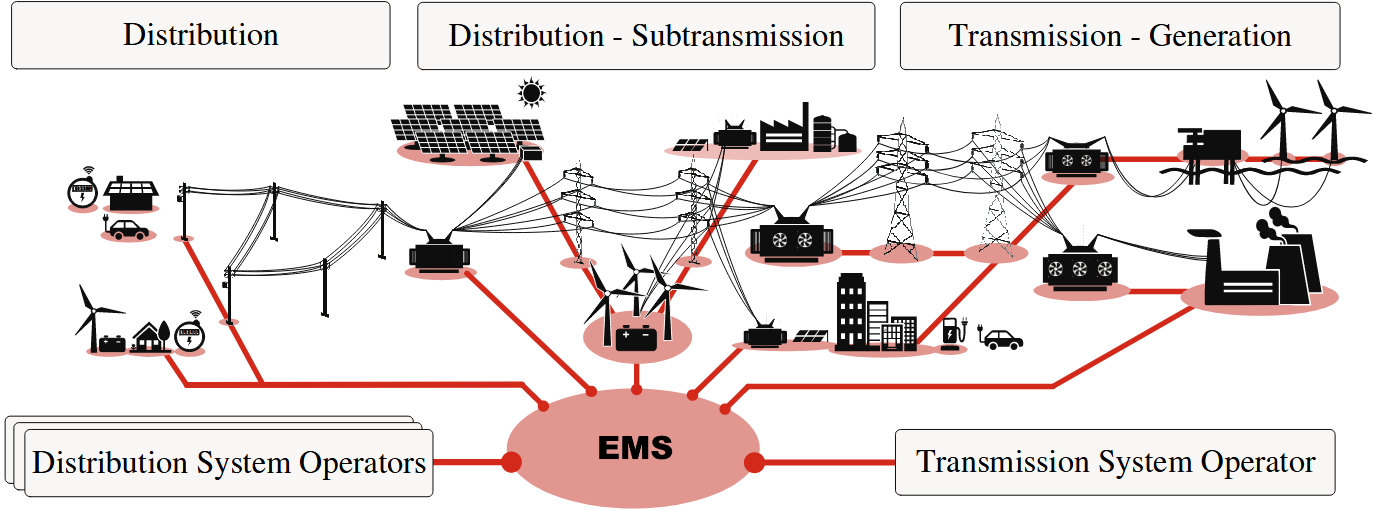
\includegraphics[scale=0.4]{ps_illustration_ems}
    }
    \caption{Illustration of modern power system \cite{Prostejovsky2017}.}\label{fig:ps_illustration}
\end{figure}

However, beyond these physical connections, maintaining secure operation critically depends on the system's overall observability. This real-time awareness of the operational state is accomplished through the deployment of numerous sensors, robust data processing infrastructure, and sophisticated information and communication technologies (ICT). The integration of the physical power infrastructure with this digital layer of monitoring and control establishes the modern power grid as a cyber-physical system. 

\nomenclature{\(ICT\)}{Information and Communication Technologies}

As the central "nerve system" of a cyber-physical entity, the Energy Management System (EMS) is designed to monitor, control, and optimize the generation, transmission, and distribution of electrical power. The State estimation (SE) serves as the fundamental element of the EMS for power networks, playing a crucial role in validating and guiding system operator decisions, including load prediction, contingency assessment, optimal power flow management, etc. SE determines the most probable voltage magnitudes and phase angles for all system buses. Accurate values are crucial for optimal and secure system operation \cite{4074022}.

% \nomenclature{\(h\)}{Planck constant}
% Обзор, введение в тему, обозначение места данной работы в
% мировых исследованиях и~т.\:п., можно использовать ссылки на~другие
% работы~\autocite{Gosele1999161,Lermontov}
% (если их~нет, то~в~автореферате
% автоматически пропадёт раздел <<Список литературы>>). Внимание! Ссылки
% на~другие работы в~разделе общей характеристики работы можно
% использовать только при использовании \verb!biblatex! (из-за технических
% ограничений \verb!bibtex8!. Это связано с тем, что одна
% и~та~же~характеристика используются и~в~тексте диссертации, и в
% автореферате. В~последнем, согласно ГОСТ, должен присутствовать список
% работ автора по~теме диссертации, а~\verb!bibtex8! не~умеет выводить в~одном
% файле два списка литературы).
% При использовании \verb!biblatex! возможно использование исключительно
% в~автореферате подстрочных ссылок
% для других работ командой \verb!\autocite!~\autocite{Marketing}, а~также цитирование
% собственных работ командой \verb!\cite!. Для этого в~файле
% \verb!common/setup.tex! необходимо присвоить положительное значение
% счётчику \verb!\setcounter{usefootcite}{1}!.

% Для генерации содержимого титульного листа автореферата, диссертации
% и~презентации используются данные из файла \verb!common/data.tex!. Если,
% например, вы меняете название диссертации, то оно автоматически
% появится в~итоговых файлах после очередного запуска \LaTeX. Согласно
% ГОСТ 7.0.11-2011 <<5.1.1 Титульный лист является первой страницей
% диссертации, служит источником информации, необходимой для обработки и
% поиска документа>>. Наличие логотипа организации на~титульном листе
% упрощает обработку и~поиск, для этого разметите логотип вашей
% организации в папке images в~формате PDF (лучше найти его в векторном
% варианте, чтобы он хорошо смотрелся при печати) под именем
% \verb!logo.pdf!. Настроить размер изображения с логотипом можно
% в~соответствующих местах файлов \verb!title.tex!  отдельно для
% диссертации и автореферата. Если вам логотип не~нужен, то просто
% удалите файл с~логотипом.

\ifsynopsis
Этот абзац появляется только в~автореферате.
Для формирования блоков, которые будут обрабатываться только в~автореферате,
заведена проверка условия \verb!\!\verb!ifsynopsis!.
Значение условия задаётся в~основном файле документа (\verb!synopsis.tex! для
автореферата).
\else
Этот абзац появляется только в~диссертации.
Через проверку условия \verb!\!\verb!ifsynopsis!, задаваемого в~основном файле
документа (\verb!dissertation.tex! для диссертации), можно сделать новую
команду, обеспечивающую появление цитаты в~диссертации, но~не~в~автореферате.
\fi

% {\progress}
% Этот раздел должен быть отдельным структурным элементом по
% ГОСТ, но он, как правило, включается в описание актуальности
% темы. Нужен он отдельным структурынм элемементом или нет ---
% смотрите другие диссертации вашего совета, скорее всего не нужен.

{\aim} данной работы является \ldots

Для~достижения поставленной цели необходимо было решить следующие {\tasks}:
\begin{enumerate}[beginpenalty=10000] % https://tex.stackexchange.com/a/476052/104425
  \item Исследовать, разработать, вычислить и~т.\:д. и~т.\:п.
  \item Исследовать, разработать, вычислить и~т.\:д. и~т.\:п.
  \item Исследовать, разработать, вычислить и~т.\:д. и~т.\:п.
  \item Исследовать, разработать, вычислить и~т.\:д. и~т.\:п.
\end{enumerate}


{\novelty}
\begin{enumerate}[beginpenalty=10000] % https://tex.stackexchange.com/a/476052/104425
  \item Впервые \ldots
  \item Впервые \ldots
  \item Было выполнено оригинальное исследование \ldots
\end{enumerate}

{\influence} \ldots

{\methods} \ldots

{\defpositions}
\begin{enumerate}[beginpenalty=10000] % https://tex.stackexchange.com/a/476052/104425
  \item Первое положение
  \item Второе положение
  \item Третье положение
  \item Четвертое положение
\end{enumerate}
В папке Documents можно ознакомиться с решением совета из Томского~ГУ
(в~файле \verb+Def_positions.pdf+), где обоснованно даются рекомендации
по~формулировкам защищаемых положений.

{\reliability} полученных результатов обеспечивается \ldots \ Результаты находятся в соответствии с результатами, полученными другими авторами.


{\probation}
Основные результаты работы докладывались~на:
перечисление основных конференций, симпозиумов и~т.\:п.

{\contribution} Автор принимал активное участие \ldots

\ifnumequal{\value{bibliosel}}{0}
{%%% Встроенная реализация с загрузкой файла через движок bibtex8. (При желании, внутри можно использовать обычные ссылки, наподобие `\cite{vakbib1,vakbib2}`).
    {\publications} Основные результаты по теме диссертации изложены
    в~XX~печатных изданиях,
    X из которых изданы в журналах, рекомендованных ВАК,
    X "--- в тезисах докладов.
}%
{%%% Реализация пакетом biblatex через движок biber
    \begin{refsection}[bl-author, bl-registered]
        % Это refsection=1.
        % Процитированные здесь работы:
        %  * подсчитываются, для автоматического составления фразы "Основные результаты ..."
        %  * попадают в авторскую библиографию, при usefootcite==0 и стиле `\insertbiblioauthor` или `\insertbiblioauthorgrouped`
        %  * нумеруются там в зависимости от порядка команд `\printbibliography` в этом разделе.
        %  * при использовании `\insertbiblioauthorgrouped`, порядок команд `\printbibliography` в нём должен быть тем же (см. biblio/biblatex.tex)
        %
        % Невидимый библиографический список для подсчёта количества публикаций:
        \phantom{\printbibliography[heading=nobibheading, section=1, env=countauthorvak,          keyword=biblioauthorvak]%
        \printbibliography[heading=nobibheading, section=1, env=countauthorwos,          keyword=biblioauthorwos]%
        \printbibliography[heading=nobibheading, section=1, env=countauthorscopus,       keyword=biblioauthorscopus]%
        \printbibliography[heading=nobibheading, section=1, env=countauthorconf,         keyword=biblioauthorconf]%
        \printbibliography[heading=nobibheading, section=1, env=countauthorother,        keyword=biblioauthorother]%
        \printbibliography[heading=nobibheading, section=1, env=countregistered,         keyword=biblioregistered]%
        \printbibliography[heading=nobibheading, section=1, env=countauthorpatent,       keyword=biblioauthorpatent]%
        \printbibliography[heading=nobibheading, section=1, env=countauthorprogram,      keyword=biblioauthorprogram]%
        \printbibliography[heading=nobibheading, section=1, env=countauthor,             keyword=biblioauthor]%
        \printbibliography[heading=nobibheading, section=1, env=countauthorvakscopuswos, filter=vakscopuswos]%
        \printbibliography[heading=nobibheading, section=1, env=countauthorscopuswos,    filter=scopuswos]}%
        %
        \nocite{*}%
        %
        {\publications} Основные результаты по теме диссертации изложены в~\arabic{citeauthor}~печатных изданиях,
        \arabic{citeauthorvak} из которых изданы в журналах, рекомендованных ВАК%
        \ifnum \value{citeauthorscopuswos}>0%
            , \arabic{citeauthorscopuswos} "--- в~периодических научных журналах, индексируемых Web of~Science и Scopus%
        \fi%
        \ifnum \value{citeauthorconf}>0%
            , \arabic{citeauthorconf} "--- в~тезисах докладов.
        \else%
            .
        \fi%
        \ifnum \value{citeregistered}=1%
            \ifnum \value{citeauthorpatent}=1%
                Зарегистрирован \arabic{citeauthorpatent} патент.
            \fi%
            \ifnum \value{citeauthorprogram}=1%
                Зарегистрирована \arabic{citeauthorprogram} программа для ЭВМ.
            \fi%
        \fi%
        \ifnum \value{citeregistered}>1%
            Зарегистрированы\ %
            \ifnum \value{citeauthorpatent}>0%
            \formbytotal{citeauthorpatent}{патент}{}{а}{}%
            \ifnum \value{citeauthorprogram}=0 . \else \ и~\fi%
            \fi%
            \ifnum \value{citeauthorprogram}>0%
            \formbytotal{citeauthorprogram}{программ}{а}{ы}{} для ЭВМ.
            \fi%
        \fi%
        % К публикациям, в которых излагаются основные научные результаты диссертации на соискание учёной
        % степени, в рецензируемых изданиях приравниваются патенты на изобретения, патенты (свидетельства) на
        % полезную модель, патенты на промышленный образец, патенты на селекционные достижения, свидетельства
        % на программу для электронных вычислительных машин, базу данных, топологию интегральных микросхем,
        % зарегистрированные в установленном порядке.(в ред. Постановления Правительства РФ от 21.04.2016 N 335)
    \end{refsection}%
    \begin{refsection}[bl-author, bl-registered]
        % Это refsection=2.
        % Процитированные здесь работы:
        %  * попадают в авторскую библиографию, при usefootcite==0 и стиле `\insertbiblioauthorimportant`.
        %  * ни на что не влияют в противном случае
        \nocite{vakbib2}%vak
        \nocite{patbib1}%patent
        \nocite{progbib1}%program
        \nocite{bib1}%other
        \nocite{confbib1}%conf
    \end{refsection}%
        %
        % Всё, что вне этих двух refsection, это refsection=0,
        %  * для диссертации - это нормальные ссылки, попадающие в обычную библиографию
        %  * для автореферата:
        %     * при usefootcite==0, ссылка корректно сработает только для источника из `external.bib`. Для своих работ --- напечатает "[0]" (и даже Warning не вылезет).
        %     * при usefootcite==1, ссылка сработает нормально. В авторской библиографии будут только процитированные в refsection=0 работы.
}

При использовании пакета \verb!biblatex! будут подсчитаны все работы, добавленные
в файл \verb!biblio/author.bib!. Для правильного подсчёта работ в~различных
системах цитирования требуется использовать поля:
\begin{itemize}
        \item \texttt{authorvak} если публикация индексирована ВАК,
        \item \texttt{authorscopus} если публикация индексирована Scopus,
        \item \texttt{authorwos} если публикация индексирована Web of Science,
        \item \texttt{authorconf} для докладов конференций,
        \item \texttt{authorpatent} для патентов,
        \item \texttt{authorprogram} для зарегистрированных программ для ЭВМ,
        \item \texttt{authorother} для других публикаций.
\end{itemize}
Для подсчёта используются счётчики:
\begin{itemize}
        \item \texttt{citeauthorvak} для работ, индексируемых ВАК,
        \item \texttt{citeauthorscopus} для работ, индексируемых Scopus,
        \item \texttt{citeauthorwos} для работ, индексируемых Web of Science,
        \item \texttt{citeauthorvakscopuswos} для работ, индексируемых одной из трёх баз,
        \item \texttt{citeauthorscopuswos} для работ, индексируемых Scopus или Web of~Science,
        \item \texttt{citeauthorconf} для докладов на конференциях,
        \item \texttt{citeauthorother} для остальных работ,
        \item \texttt{citeauthorpatent} для патентов,
        \item \texttt{citeauthorprogram} для зарегистрированных программ для ЭВМ,
        \item \texttt{citeauthor} для суммарного количества работ.
\end{itemize}
% Счётчик \texttt{citeexternal} используется для подсчёта процитированных публикаций;
% \texttt{citeregistered} "--- для подсчёта суммарного количества патентов и программ для ЭВМ.

Для добавления в список публикаций автора работ, которые не были процитированы в
автореферате, требуется их~перечислить с использованием команды \verb!\nocite! в
\verb!Synopsis/content.tex!.
